%begin{document}

\section{Workplace environment management}
\label{47}

\subsection{Temperature and relative humidity}
\subsubsection{Data}
Air temperatures and relative humidity measured are presented in Table \ref{ch047_tbl_tdb_rh}. Data was measured at targeted points shown in Figure \ref{fig_ch02_wem01}. Raw data is with the site inspection reports, which will be provided to the Client separately. Persuant to ASHRAE standard, the recommended ranges for temperature and humidity are [72 - 80 $^\circ F$] and [45 - 60 \%], respectively.

\subsubsection{Data and Analysis}

\begin{table}
	\caption{Temperature and Relative Humidity}
	\label{ch047_tbl_tdb_rh}
	{\footnotesize

\begin{tabular}{l|c|c|c|c}

\hline
Description of Location & \multicolumn{1}{c}{Temperature} &  & \multicolumn{1}{c}{RH} &  \\ 
\cline{2-5}
 & Actual & Range & Actual & Range \\ 
\hline
A &  &  &  &  \\ 
Beside P4 & 84.2 & 72-80 & 66.3 & 45-60 \\ 
At staging area opposite 1 & 84.0 & 72-80 & 66.6 & 45-60 \\ 
Between P3 and P4 & 83.8 & 72-80 & 67.2 & 45-60 \\ 
Near MCC opposite 3 & 83.8 & 72-80 & 67.9 & 45-60 \\ 
Between P2 and P3 & 83.8 & 72-80 & 68 & 45-60 \\ 
Near MCC opposite5 & 83.5 & 72-80 & 66.3 & 45-60 \\ 
Between P1 and P2 & 84.4 & 72-80 & 65.4 & 45-60 \\ 
Near MCC opposite 7 & 84.0 & 72-80 & 65.4 & 45-60 \\ 
Beside P1 & 84.6 & 72-80 & 65.5 & 45-60 \\ 
Near door 3 opposite 9 & 84.6 & 72-80 & 64.4 & 45-60 \\ 
Average & 84.1 & 72-80 & 66.3 & 45-60 \\ 
\hline
B &  &  &  &  \\ 
Open area beside pump room & 33.2 & 72-80 & 56.1 & 45-60 \\ 
Open area beside pump room & 32.1 & 72-80 & 59.3 & 45-60 \\ 
Average & 32.7 & 72-80 & 57.7 & 45-60 \\ 
\hline
C &  &  &  &  \\ 
Comfort room & 30.1 & 72-80 & 62.7 & 45-60 \\ 
Office & 30.5 &  & 64.2 &  \\ 
Average & 30.3 & 72-80 & 63.5 & 45-60 \\ 
\hline
D &  &  &  &  \\ 
Near Guard house & 30.8 & 72-80 & 61.3 & 45-60 \\ 
\hline

\end{tabular}
}
\end{table}

The pump station is situated near dense forestry and is connected to the subdivision roads via an access road. There are no significant sources of pollution and almost no passersby.  
As an old pump station building, there is no mechanical air conditioning. The pump room relies on natural ventilation via the access door and room windows. The MCC room beside the pump room is also naturally ventilated and has windows installed. Air properties are similar for all the areas in the station. From the table, the temperatures inside the pump house at every measurement points are significant higher than the maximum value of the recommended range (80 F). The average value is around 87 F. High values of temperature compared to the range have also been observed for points outside the pump house. The same is observed for the values of RH.

Solar load on the operators room is high during the day until noon (Figure \ref{fig_ch047_wem_optr_room} - a) and is low for the afternoon. To avoid consistent exposure to heat, the operator can stay on the shaded areas for cooling where the guard’s booth is also positioned. Thus, comfort is sought of by the operator by feel and by shading himself when especially when the sun is up. 

In terms of operatorship, there is not much significance deviation of the readings from recommended range since the operator spends small amount of time intermittently to record information or to start or stop the pumps during his shift.

Nonetheless, temperature and humidity are correlated and as per ASHRAE standard 55 under summer comfort zone, the recommended combination of temperature and humidity shall be within the comfortable zone as shown in Figure \ref{fig_ch047_ashrae_psychrometrics}.

\begin{figure}[!htb]
	\includegraphics[scale=2]{figures/fig_ch047_ashrae_psychrometrics} \\
	\caption{ASHRAE standard 55 : Summer Comfort Zone}
	\label{fig_ch047_ashrae_psychrometrics} 
\end{figure} 

\subsubsection{Recommendations}
In order to reduce the negative impacts from high temperature, particularly inside the pump house, the Client shall consider

\begin{itemize}
	\item Establishing a good daily monitoring, exercise, and management considering ergonomic and health and occupational activities (e.g. appropriate time window for break in designated resting area);.
	\item Transfer operators room or refurbish existing room to negate heat especially during day.
	\item Install AC equipment at least for the MCC room where cool air is desired to help MCC function efficiently and safely.  
\end{itemize}

\subsection{Air quality}\label{aq01}

\subsubsection{Data and analysis}
Air particulate matter concentrations are presented in Table \ref{ch047_tbl_pm.txt}. Data was measured at targeted points shown in \ref{fig_ch02_wem01}. Raw data is with the site inspection reports, which will be provided to the Client separately. Pursuant to currently applied standard, excellent air quality range for PM2.5 is in [0-35].

\begin{table}
	\caption{Air Quality - PM2.5}
	\label{ch047_tbl_pm}
	{\footnotesize
\begin{tabular}{c|l|c}

\hline
Point & Description of Location & PM2.5 \\ 
\hline
A &  &  \\ 
1 & Beside P4 & 10 \\ 
2 & At staging area opposite 1 & 10 \\ 
3 & Between P3 and P4 & 10 \\ 
4 & Near MCC opposite 3 & 10 \\ 
5 & Between P2 and P3 & 9 \\ 
6 & Near MCC opposite5 & 10 \\ 
7 & Between P1 and P2 & 9 \\ 
8 & Near MCC opposite 7 & 10 \\ 
9 & Beside P1 & 9 \\ 
10 & Near door 3 opposite 9 & 9 \\ 
 & Average & 9.6 \\ 
\hline
B &  &  \\ 
11 & Open area beside pump room & 10 \\ 
12 & Open area beside pump room & 10 \\ 
 & Average & 10.0 \\ 
\hline
C &  &  \\ 
13 & Comfort room & 8 \\ 
14 & Office & 8 \\ 
 & Average & 8.0 \\ 
\hline
D &  &  \\ 
15 & Near Guard house & 10 \\ 
\hline

\end{tabular}
}
\end{table}

The air quality for the pump station in terms of particulate matter is excellent. This is simply because there are no nearby significant sources of pollution such as emissions from vehicles for pump stations situated near heavy traffic roads.


\subsubsection{Recommendations}

Follow strictly safety and environmental regulation. For example, all employees and staff to wear appropriate dust-proofed masks when working with activities that potentially incurs dusts or other harmful particles.



%\subsection{Hazards}\label{aq02}
%\textcolor{red}{RB Sanchez to write here the summary of raw data collected from visual inspection and testing. Tables shall be used as much as we can. Note that no analysis in this session. This session is purely the high level presentation of data. Raw data can be linked as an Appendix}
\subsection{Illumination}\label{aq03}
\subsubsection{Data and analysis}
Illumination within various areas of the pump station are presented in Table \ref{ch047_tbl_illumination} with the LUX value. Data was measured at targeted points shown in Figure \ref{fig_ch02_wem01}. Raw data is with the site inspection reports, which will be provided to the Client separately. Persuant to RULE 1075.4 of DOLE-OSH standard \cite{DOLE2016}, the recommended minimum for LUX is in 100.

\begin{table}
	\caption{Illumination}
	\label{ch047_tbl_illumination}
	{\footnotesize


\begin{tabular}{c|l|c}
\hline
Point & Description of the Point Location & Illumination \\ 
\hline
 & A. &  \\ 
1 & Pump 1  (near storage) & 18 \\ 
2 & Pump 1  (near door) & 106 \\ 
3 & Pump 2 (near storage) & 280 \\ 
4 & Pump 2  (near door) & 18 \\ 
5 & Pump 3  (near storage) & 82 \\ 
6 & Pump 3 (below) & 16 \\ 
7 & Between pump 1 and 2 (below) & 18 \\ 
8 & Between pump 1 and 2 (near storage) & 250 \\ 
 & Average & 94.3 \\ 
\hline
 & B. &  \\ 
9 & Office & 340 \\ 
10 & Electrical room & 320 \\ 
 & Average & 330 \\ 
\hline
 & C. &  \\ 
11 & Parking lobby access (between generator and electrical room) & 6900 \\ 
12 & Payment center outside area & 4200 \\ 
13 & Payment center outside area (left side) & 7500 \\ 
14 & Reservoir left side corner & 1800 \\ 
15 & Reservoir right side corner (near day tank) & 106000 \\ 
16 & Reservoir right side corner (near parking lot) & 7400 \\ 
17 & Outer area near pump room & 2400 \\ 
 & Average & 19457 \\ 
\hline
\end{tabular}
}
\end{table}

Illumination levels measured are above recommended minimum. The pump station is mostly solar lit during the day thru door and windows (Figure \ref{fig_ch047_wem_window}). Lightings can provide necessary illumination if brighter working area is needed, especially during afternoon and evenings. Concern is raised for evening or graveyard shifts where the operator needs to inspect around the reservoir area. Ample lighting is desired to help operator safely roam and inspect the area. 


\subsubsection{Recommendations}

\begin{itemize}
	\item	Install necessary lighting along path to reservoir and vicinity 
	
\end{itemize}


\subsection{Industrial ventilation}\label{aq04}
\subsubsection{Data and analysis}

The pump room relies on natural ventilation via the access door and room windows. The MCC room beside the pump room is also naturally ventilated and has windows installed. The open access doors and windows serve double purpose to both promote air change in the rooms and also provide natural lighting inside (Figure \ref{fig_ch047_wem_window})

\begin{figure}[!htb]
	\begin{minipage}[b]{0.225\linewidth}
		\centering
		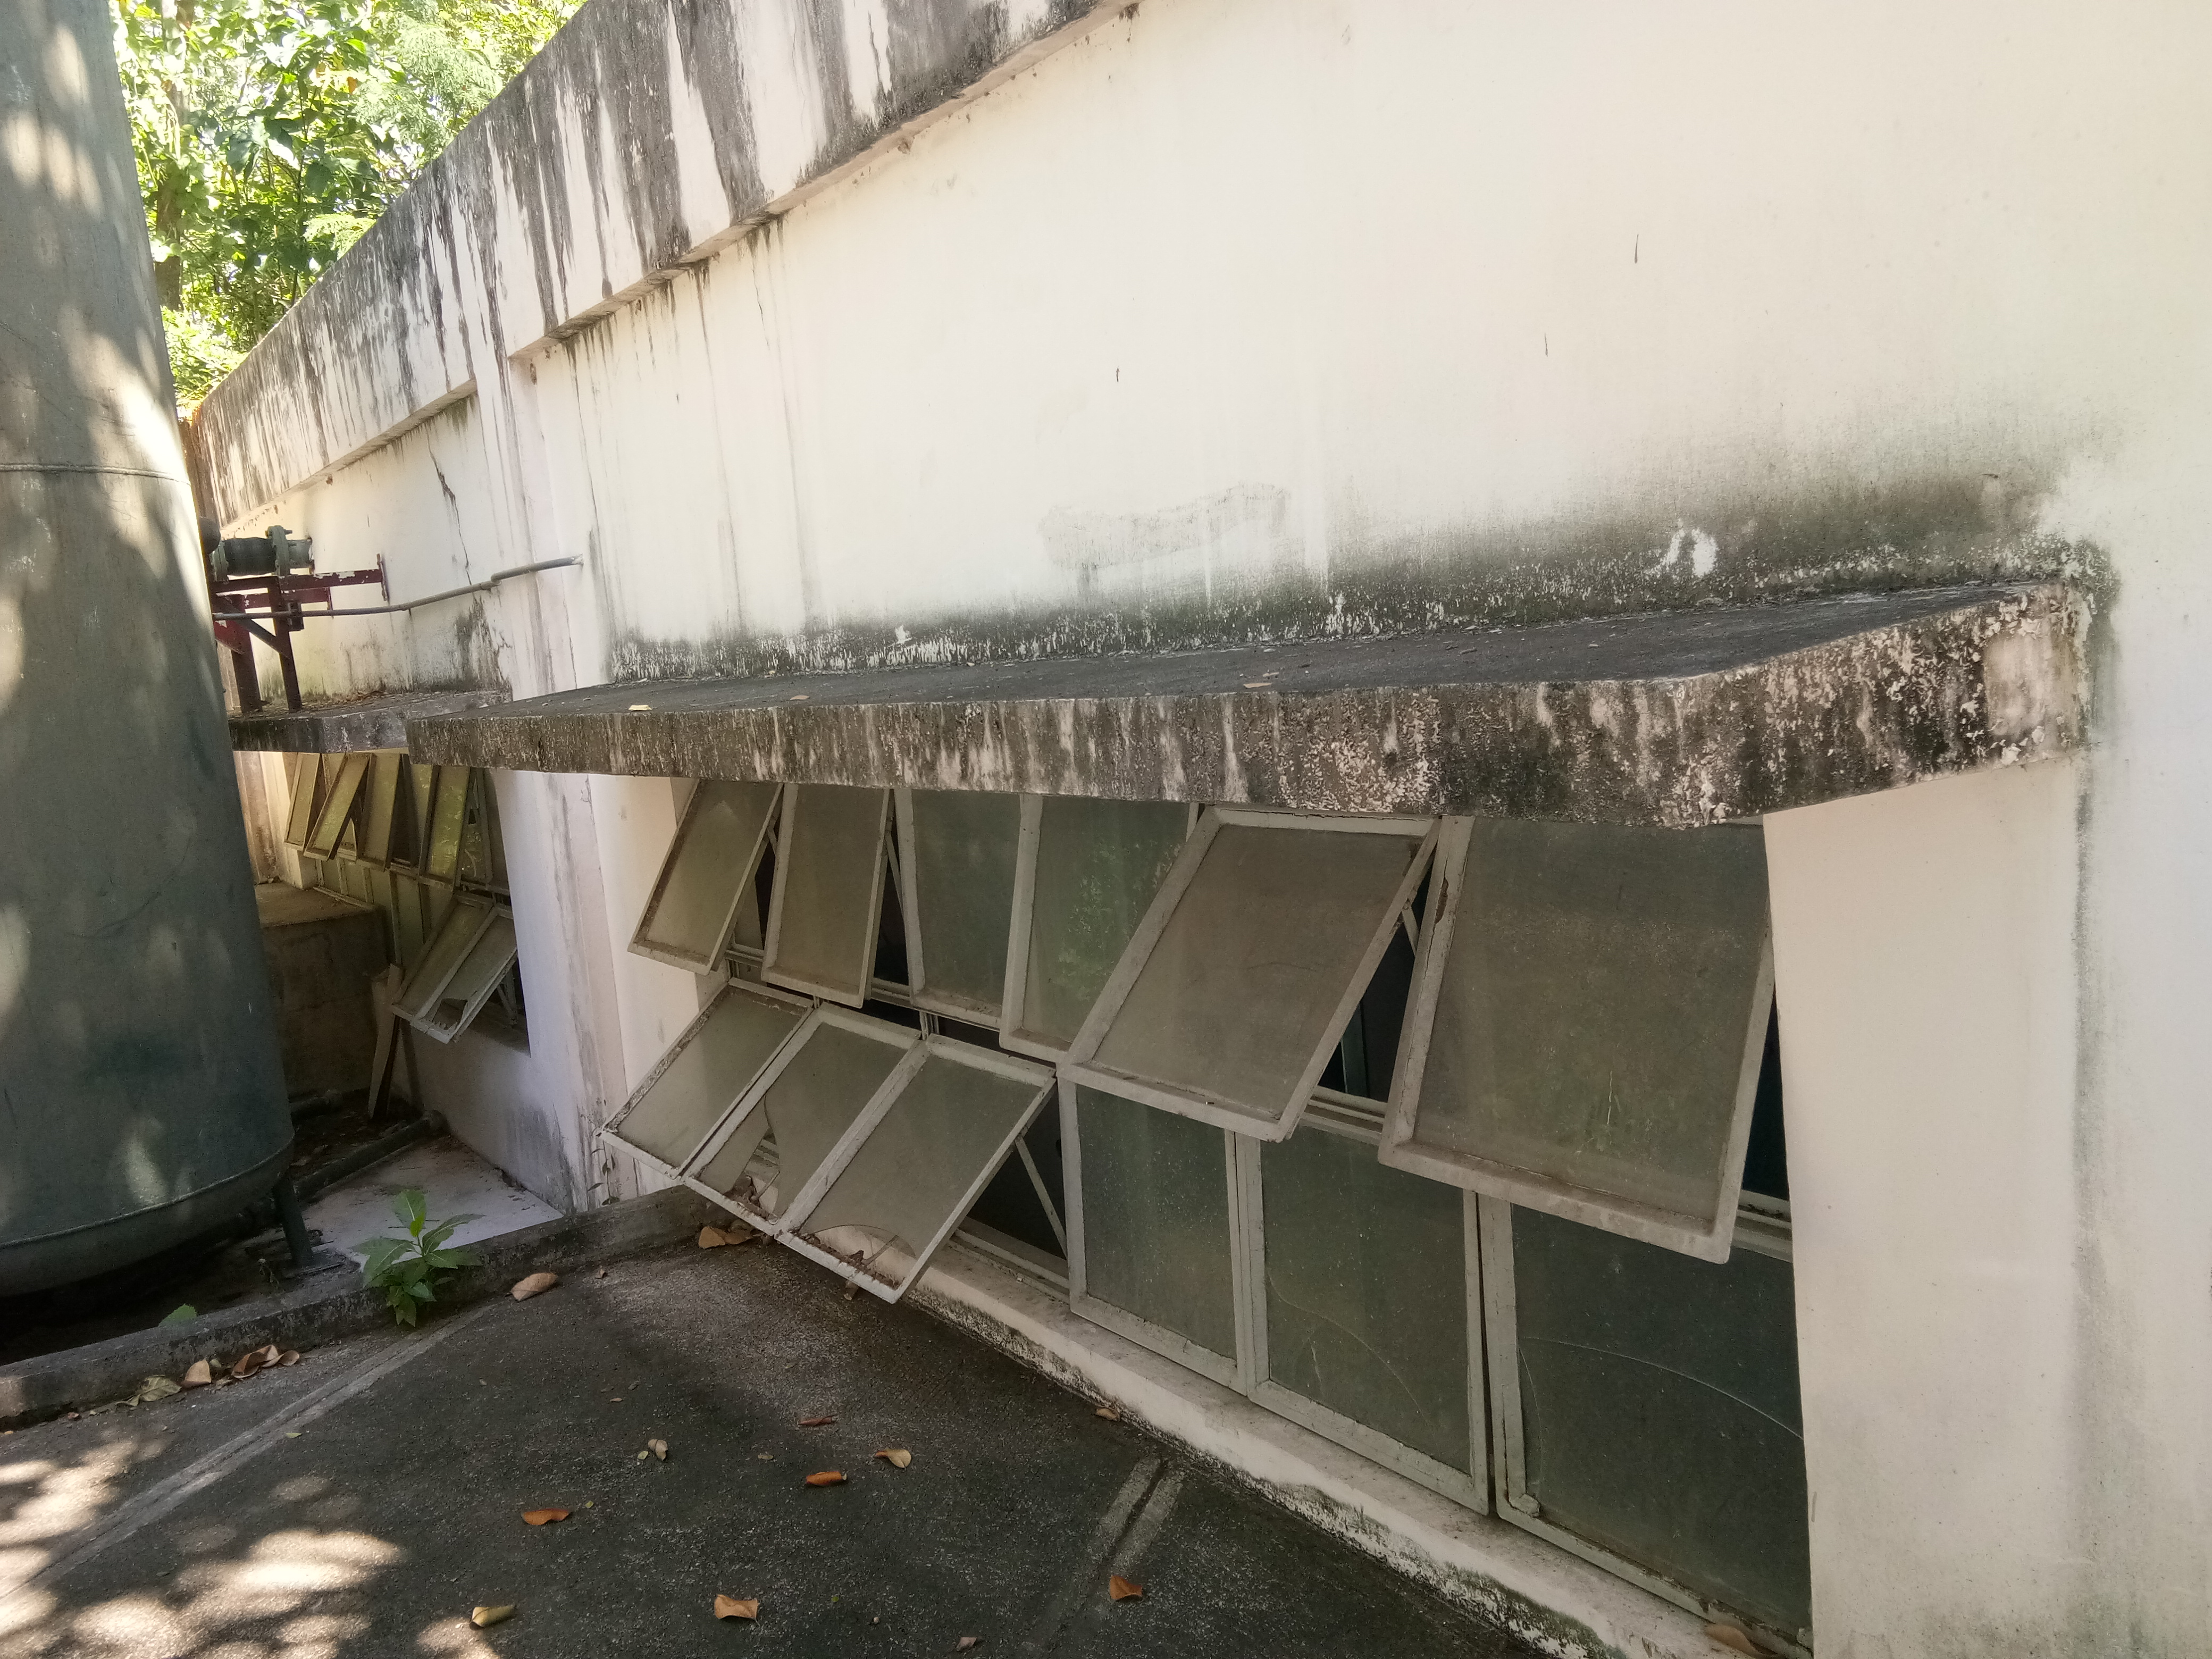
\includegraphics[width=\textwidth]{figures/fig_ch047_wem_window_illu}
		\caption*{a}
		%		\label{pagcorlocation}
	\end{minipage}
	\hspace{0.05cm}
	\begin{minipage}[b]{0.225\linewidth}
		\centering
		\includegraphics[width=\textwidth]{figures/fig_ch047_wem_illuA}
		\caption*{b}
		%		\label{ch01_pumpgallery}
	\end{minipage}
	\hspace{0.05cm}
	\begin{minipage}[b]{0.225\linewidth}
		\centering
		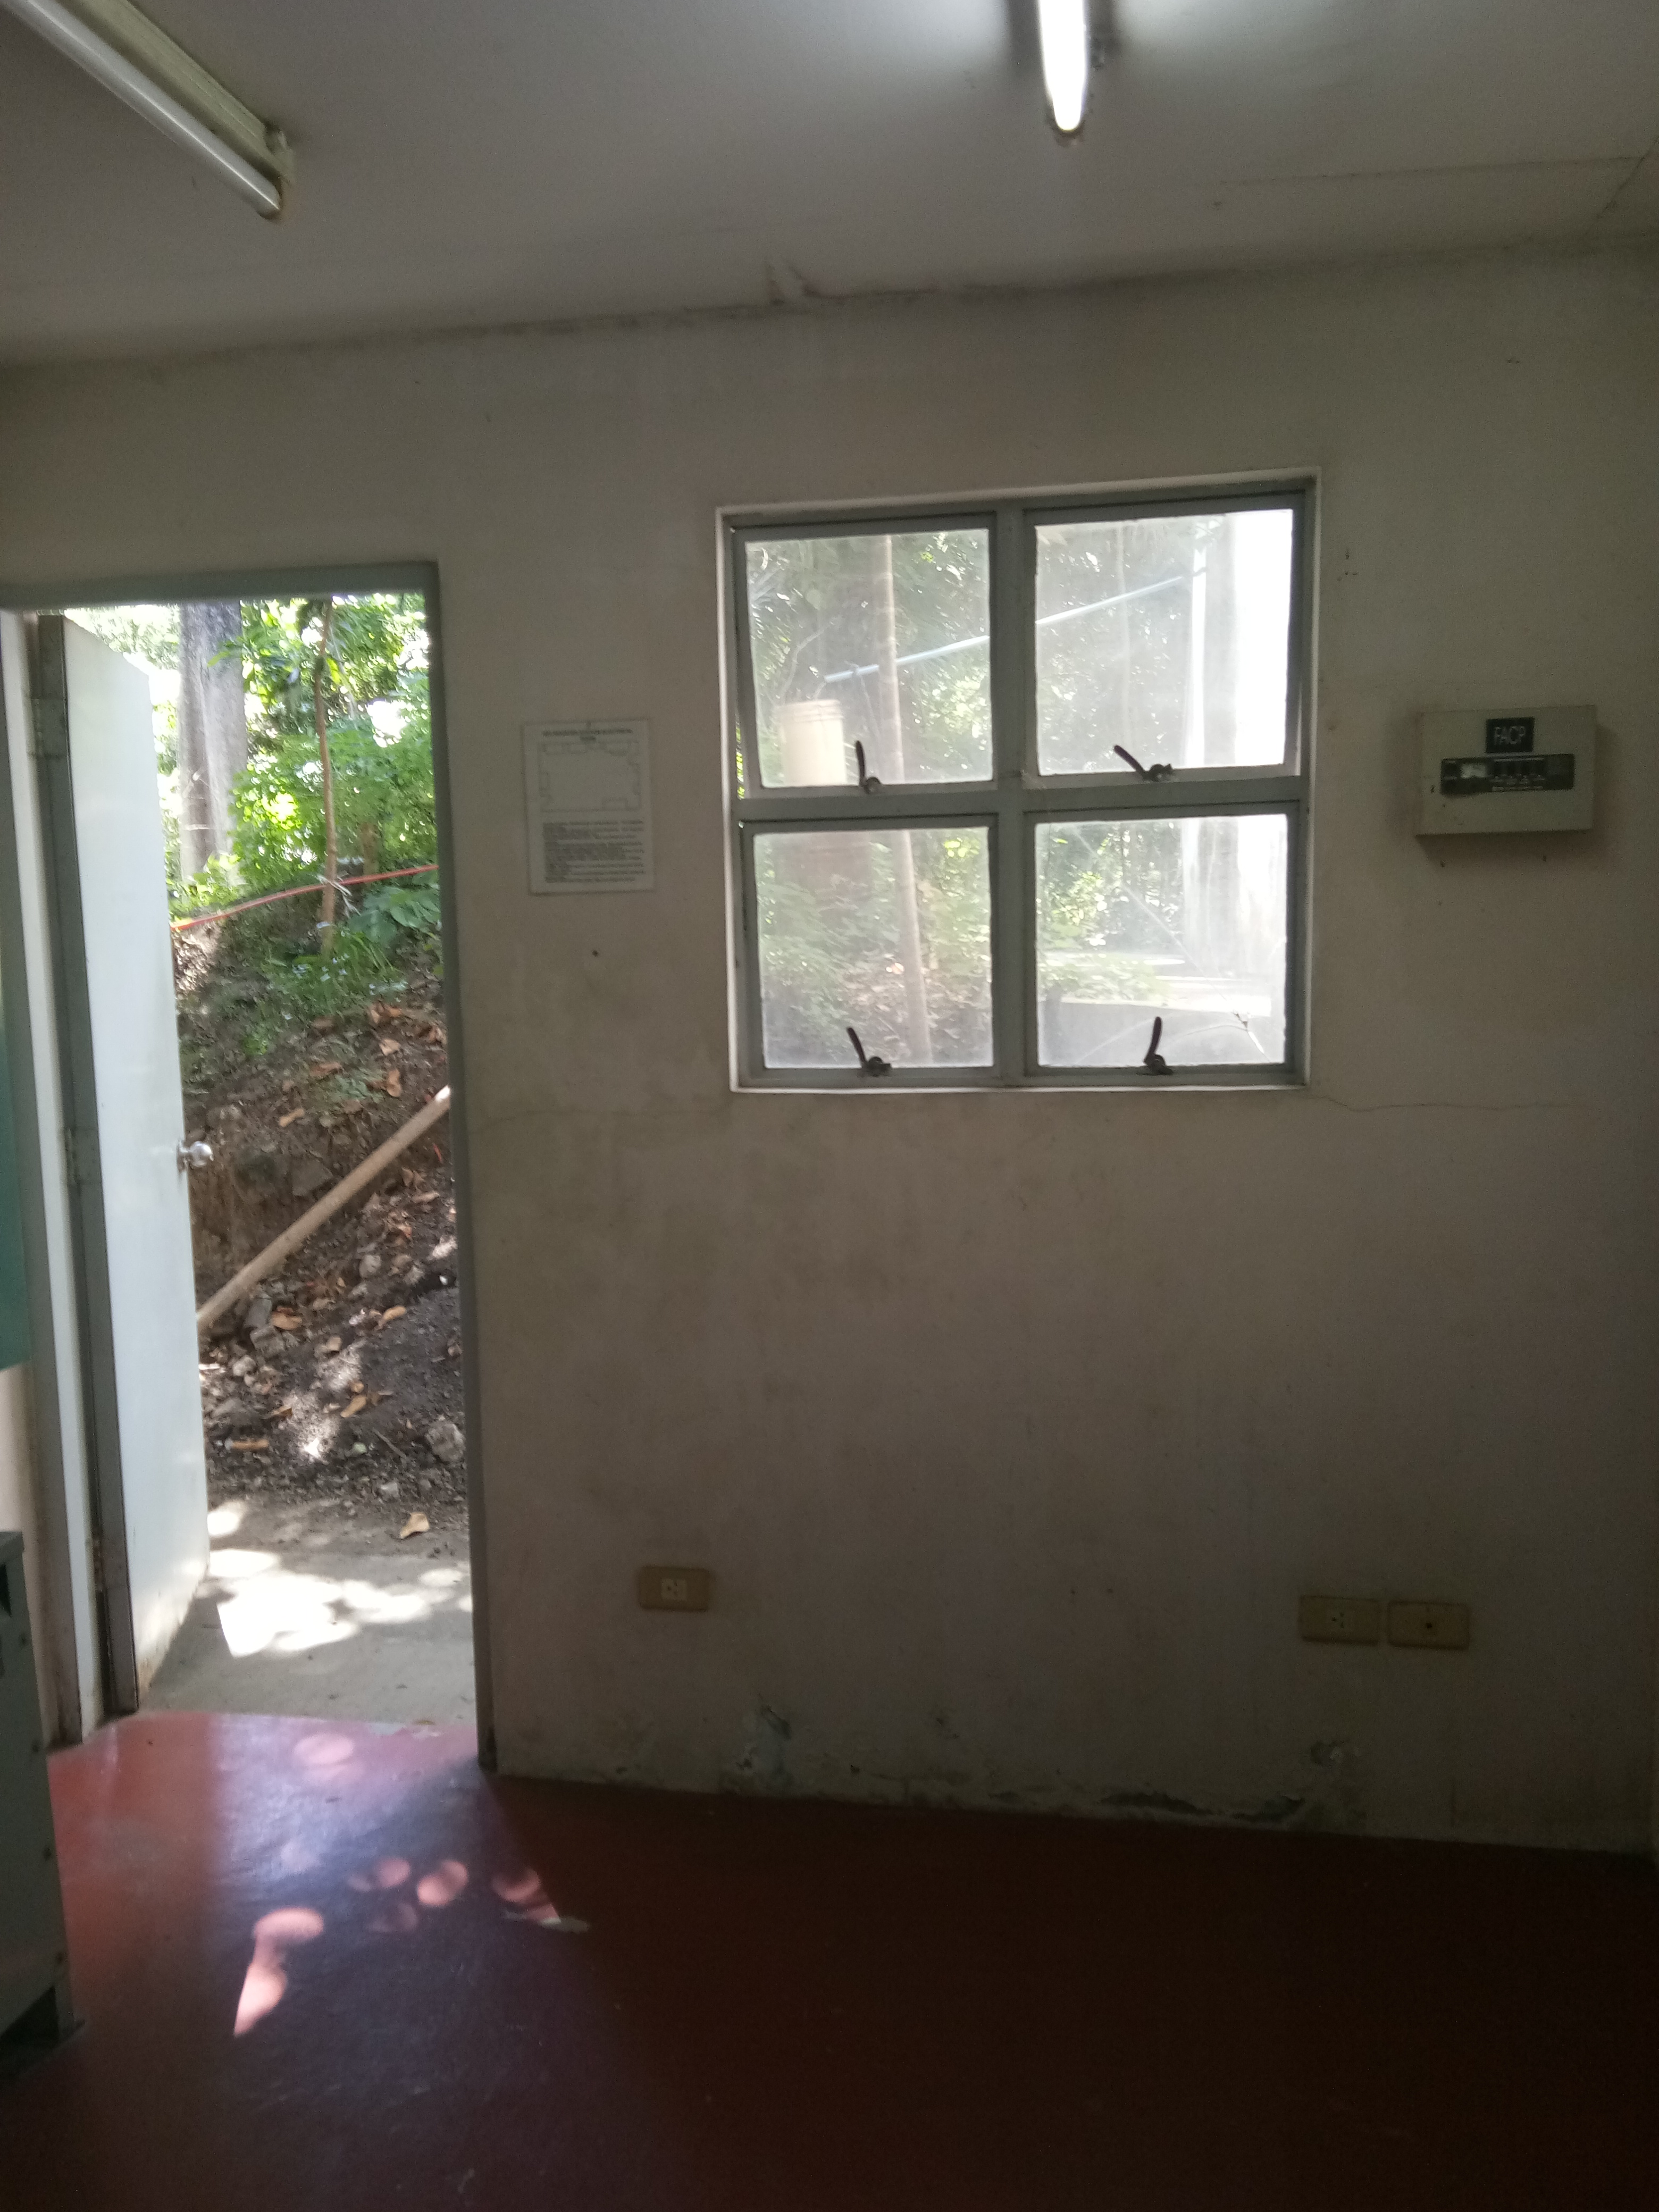
\includegraphics[width=\textwidth]{figures/fig_ch047_wem_openings}
		\caption*{c}
		%		\label{ch01_pumpgallery}
	\end{minipage}
	\hspace{0.05cm}
	\begin{minipage}[b]{0.225\linewidth}
		\centering
		\includegraphics[width=\textwidth]{figures/fig_ch043_illus}
		\caption*{d}
		%		\label{ch01_pumpgallery}
	\end{minipage}
	\caption{Pump house openings}
	\label{fig_ch047_wem_window}
\end{figure}

%Recommendation for ventilation needed
%\begin{figure}[h]
%\includegraphics[scale=0.6]{figures/ch047_wem_ventilation} \\
%	\caption{Existing ventilation layout}
%	\label{ch047_wem_ventilation} 
%\end{figure}


\subsubsection{Recommendations}

\begin{itemize}
	\item No action needed.
\end{itemize}

\subsection{Housekeeping}\label{aq05}
\subsubsection{Documentation}
Following problems are the facts:

\begin{itemize}
	\item Current documentation practice is heavily dominated with paper based system, which follows the current practice in Maynilad. There is a large amount/collection of papers that recorded past activities but is of no use and beneficial if data cannot be transformed into digital format for time series analysis, which is an essential part of asset management practice;
	
	\item No proper filing/library system with standardized coding rule that will provide convenience for operators/users to timely find appropriate documents;
	
	\item Daily operation data is crucial information for future analysis but it is recorded in excel based file without relational tables, which makes it from hard to impossible for data compilation, filtering, and mining. Many past data has been recorded with outliers and incorrect data types. 
	
\end{itemize}

\subsubsection{Waste management and environmental control}
There is no issue with regard to waste management and environmental control as confirmed by the checklist shown in Table \ref{ch047_tbl_housekeeping}

\begin{table}
	\caption{Housekeeping.}
	\label{ch047_tbl_housekeeping}
	{\footnotesize

\begin{tabular}{p{4cm}|c|c|c|p{6cm}}
\hline
Description & Status & CS & IT & Remarks \\ 
\hline
Pump room cleanliness & yes & 1 & 1 & After maintenance or intervention, area should be thoroughly cleaned. Water sumps be dried and grease be wiped \\ 
Sufficient waste segregation assets & yes & 1 & 1 &  \\ 
Waste segregation policy & yes & 1 & 1 &  \\ 
Proper/ appropriate signage & yes & 1 & 1 &  \\ 
Genset emission control & yes &  & 1 &  \\ 

\hline
\end{tabular}
	}
\end{table}


%The plant has its own waste segregation policy and an organized documentations procedure (evidenced of the arranged daily monitoring sheet). Standby generator set is situated outside the pump house where its exhaust gases through natural ventilation will not be able to penetrate the pump house.

\subsubsection{Office arrangement and ergonomic}
Table \ref{ch047_tbl_ergonomics} shows the data concerning parameters associated with office arrangement and ergonomic considerations.

\begin{table}[!h]
	\caption{Ergonomics.}
	\label{ch047_tbl_ergonomics}
	{\footnotesize


\begin{tabular}{p{1.5cm}|p{1.5cm}|c|p{8.5cm}}
\hline
Parameters & Sub-parameters & Status & Remarks \\ 
\hline
Posture & Head & 1 & Ceiling height is high enough to cause head injury while sitting or when standing. \\ 
 & Neck & 1 & Neck posture is in good ergonomic condition. \\ 
 &  &  & Consider having an interval for fit-break to avoid neck muscles stiffening. \\ 
 & Back & 1 & Back posture while sitting is in good posture.  \\ 
 &  &  & Consider standing and doing fit-break exercises to relax spine.  \\ 
 & Hands/Wrist  & 0 & Proper hand positioning in the keyboard is not observed. \\ 
 &  &  & Wrist bending is seldom. \\ 
 & Feet & 1 & Feet position is in good posture. \\ 
 &  &  & Good clearance below worktables. \\ 
 & Eyes & 0 & The computer monitor is on eyelevel in a certain operator only. \\ 
 &  &  & Consider adjusting the monitor level comfortable to every operator. \\ 
 &  &  & Look away into distance in order to rest the eyes for every 10 minutes or so. \\ 
\hline
Equipment / Tool &  &  &  \\ 
 & Computer display & 0 & Not adjusted and the operator get used to its current setting. \\ 
 &  &  & Display brightness must be adjustable in the comfortability of the operator-in-charge. \\ 
 &  &  & Consider the use of anti-glare and blue light to reduce the possibility of eyestrain. \\ 
 & Keyboard & 1 & Keyboard position causes poor hand posture that can lead to injury at long exposure. \\ 
 & Mouse & 1 & Mouse usage is average due to monitoring. \\ 
 &  &  & Prolong usage may cause reduced blood flow leading to muscular injury. \\ 
 & Chair & 0 & Consider using ergonomic chair that is capable of back support, height, armrest adjustments. \\ 
 & Table & 0 & Consider use of ergonomic tables to adjust the height of the table in desired position easily without exerting much effort to adjust manually. \\ 
 & Files & 1 & Hard copy file system and location is well observed. Too high or too low file location may require a person to bend his body or force his hand to grip a file in an awkward posture. Frequent situation may lead to MSD. \\ 
\hline
Operations / Maintenance & Illumination & 0 & According to the maintenance team, the motion-activated light is not bright enough to complete their task efficiently at night. Moreover, the light has short on-off delay operation that means that the team must move more often to avoid the light to dim.  \\ 
 &  &  & Consider having a manual switch option to by-pass the motion sensors and le the light on while doing maintenance.  \\ 
 & Noise Exposure & 1 & Noise emitted by the machines in the pump station is high. Consider the use of proper ear protections to reduce the sound intensity. In offices, the sound intensity is acceptable.  \\ 
 & Temperature & 1 & Temperature in the pump station is not acceptable at long exposure. Consider cooling down the body temperature at the designated area (i.e. outside, office). \\ 
\hline
Facility / General Workplace & Layout & 1 & Layout of the pump station is well observed. Distance between pumps is acceptable for well maintenance movement.  \\ 
 & Height clearances & 1 & Height clearances from ceiling to head is very high. Chance of getting head injury is very low. \\ 
\hline
\end{tabular}

	}
\end{table}


%\begin{table}[h]
    \caption{Housekeeping}
    \label{ch05_tbl_housekeeping}
    \footnotesize{

\begin{tabular}{l|c|c|c|l}
\hline
Description & Status & CS & IT & Remarks \\ 
\hline
- Sufficient waste segregation assets & yes & 1 & 1 &  \\ 
- waste segregation policy & yes & 1 & 1 &  \\ 
- Signage & yes & 1 & 1 &  \\ 
- Genset emission control & yes &  & 1 &  \\ 
\hline
\end{tabular}
}

\end{table}


\subsubsection{Recommendations}
Followings are recommendations

\begin{itemize}
	\item Development of a web-based database management system, with appropriate set of relational data tables to record operational data, power consumption data, and intervention data;
	
	\item Development of documentation code and naming for appropriate filing and library/referencing;
	
	\item Refurbish operator’s office (Figure \ref{fig_ch047_wem_optr_room} - b) and include necessary organizing items such as file cabinet 
	
\end{itemize}

\begin{figure}[!htb]
	\begin{minipage}[b]{0.4\linewidth}
		\centering
		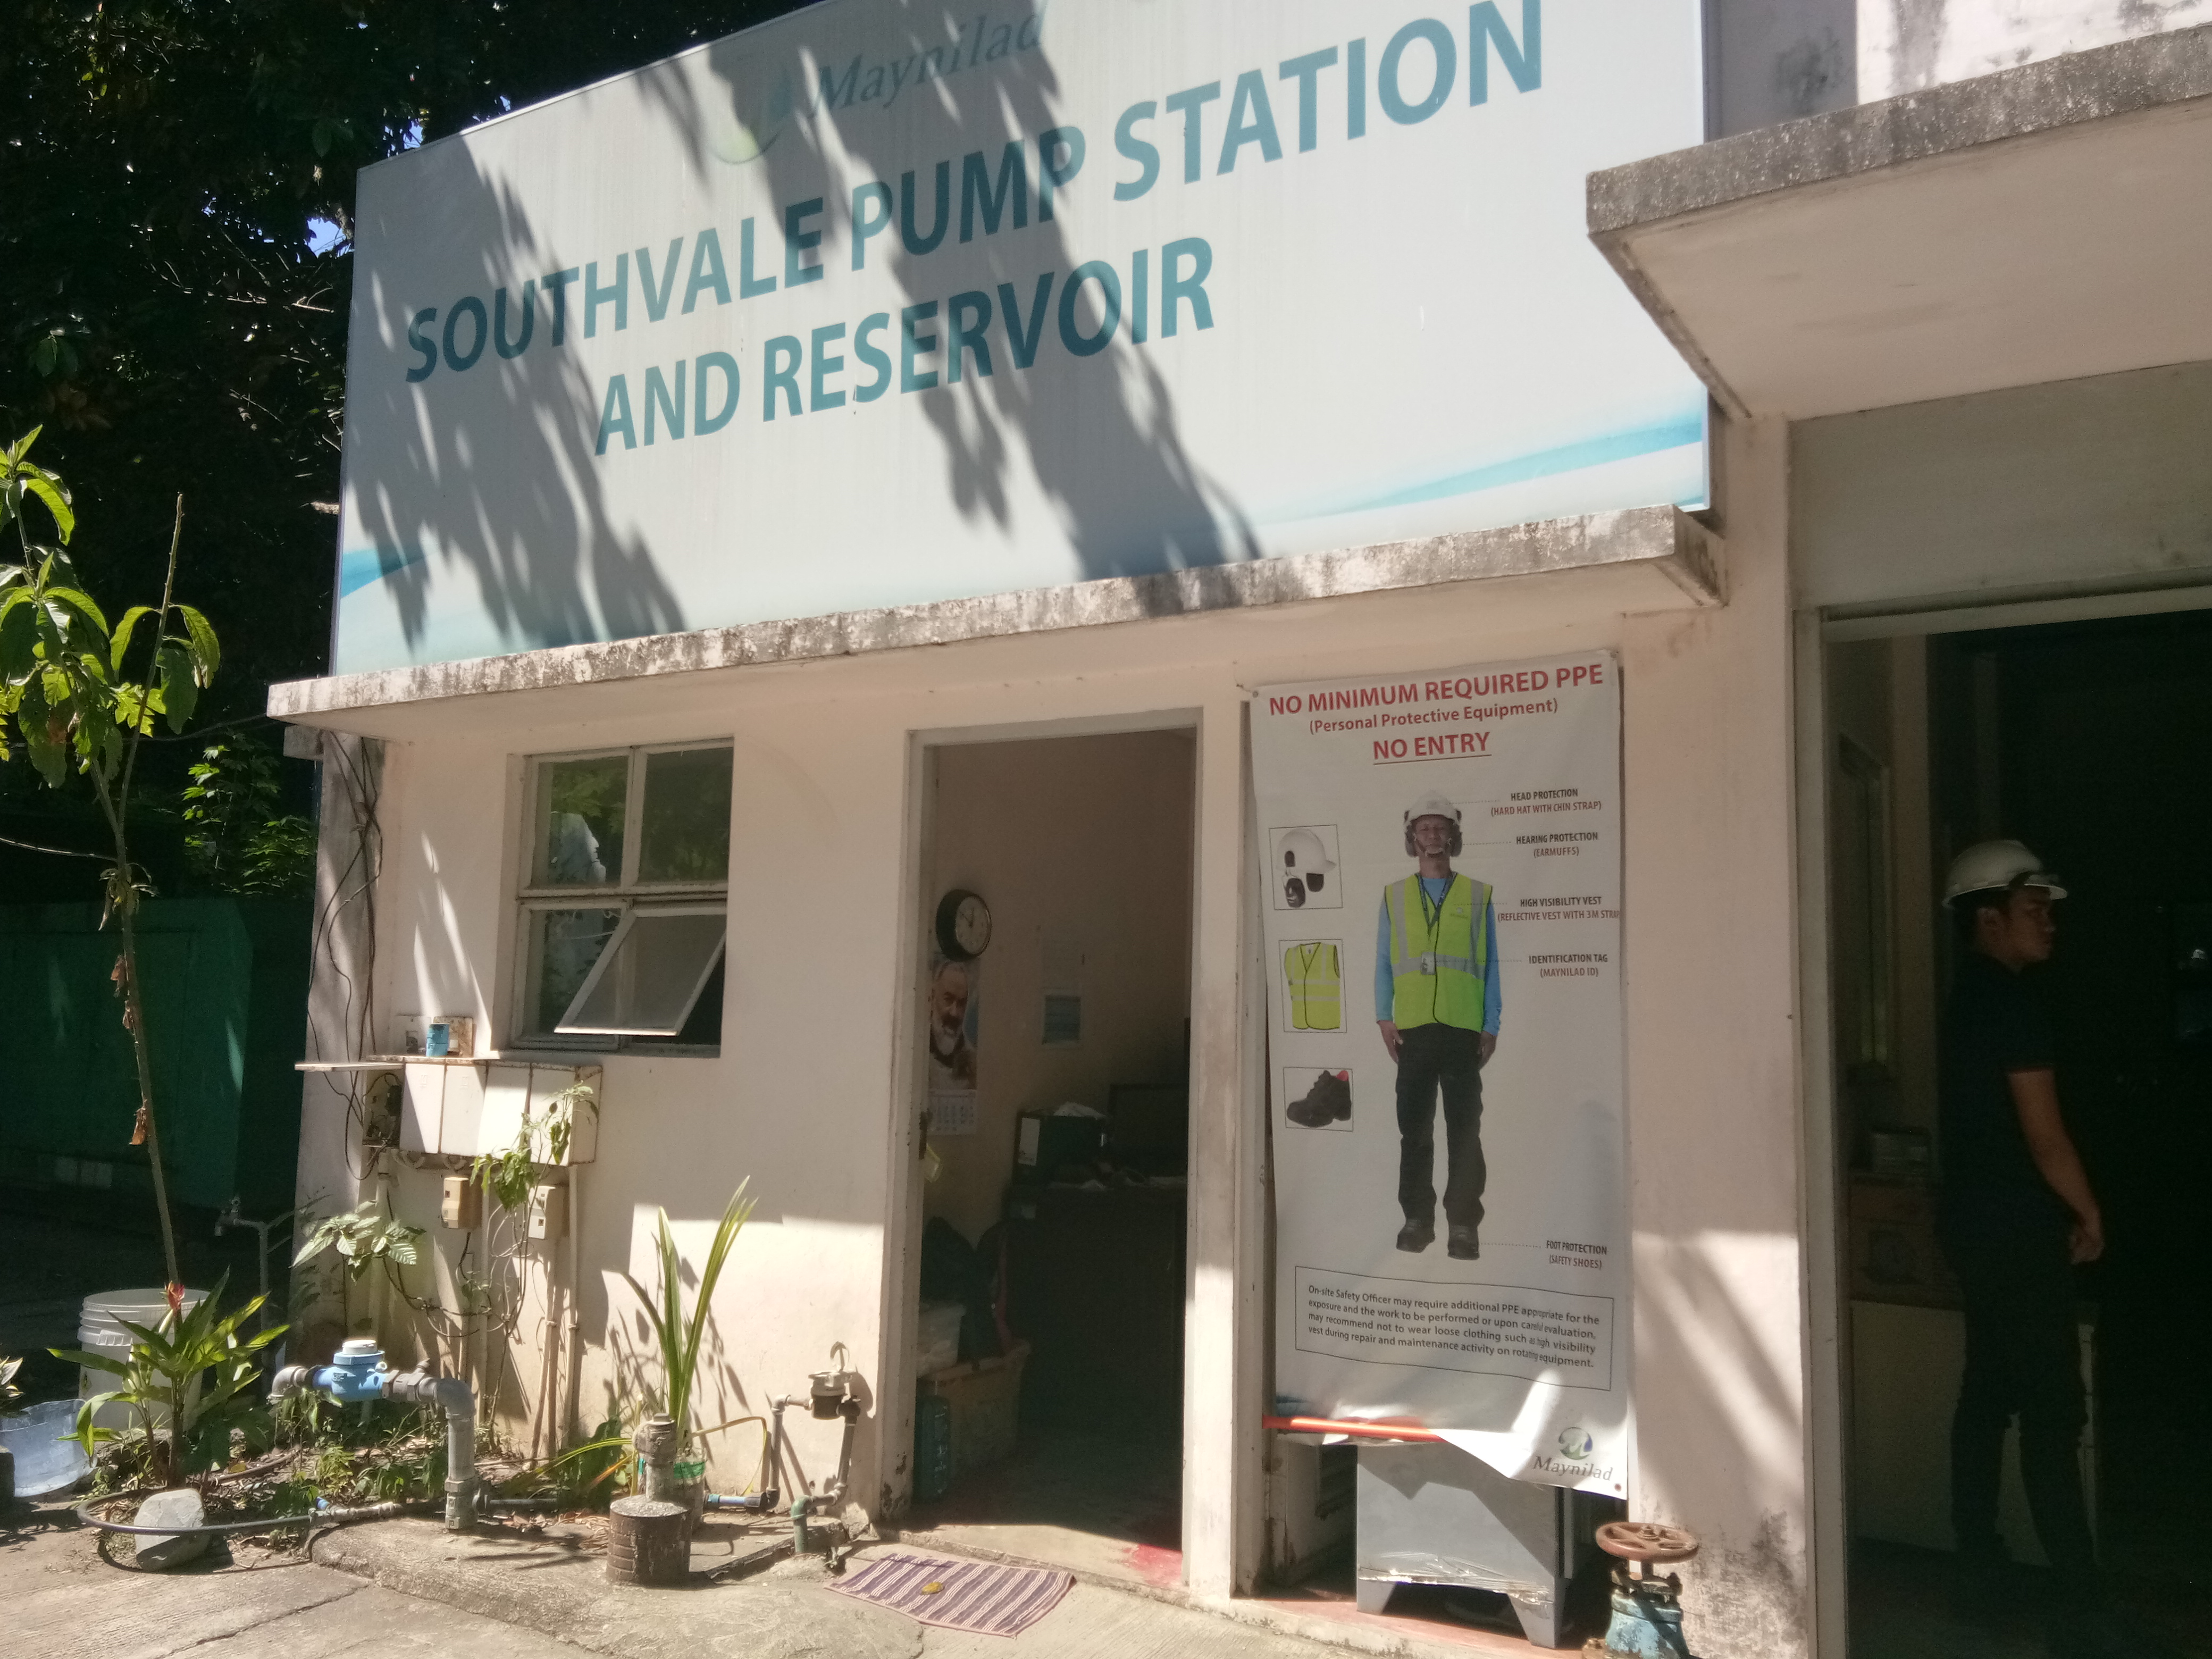
\includegraphics[width=\textwidth]{figures/fig_ch047_wem_optr_room}
		\caption*{a - High solar load during the day}
		%		\label{pagcorlocation}
	\end{minipage}
	\hspace{0.05cm}
	\begin{minipage}[b]{0.225\linewidth}
		\centering
		\includegraphics[width=\textwidth]{figures/fig_ch047_wem_optrsdesk}
		\caption*{b - Operator's desk}
		%		\label{ch01_pumpgallery}
	\end{minipage}
	\caption{Operator's room}
	\label{fig_ch047_wem_optr_room}
\end{figure}

\subsection{Noise}\label{aq06}
\subsubsection{Data and analysis}
Sound level measurements are presented in Table \ref{ch047_tbl_sound}. Data was measured at targeted points shown in Figure \ref{fig_ch02_wem01}. Raw data is with the site inspection reports, which will be provided to the Client separately.  

\begin{table}
	\caption{Sound Levels.}
	\label{ch047_tbl_sound}
	{\footnotesize

\begin{tabular}{c|l|c}
\hline
Point & Description of the Point Location & Sound level \\ 
\hline
 & A. &  \\ 
1 & Pump 1  (near storage) & 95.8 \\ 
2 & Pump 1  (near door) & 93.8 \\ 
3 & Pump 2 (near storage) & 93.2 \\ 
4 & Pump 2  (near door) & 94.2 \\ 
5 & Pump 3  (near storage) & 90.5 \\ 
6 & Pump 3 (below) & 94.2 \\ 
7 & Between pump 1 and 2 (below) & 96.9 \\ 
8 & Between pump 1 and 2 (near storage) & 95.7 \\ 
 & Average & 94.3 \\ 
\hline
 & B. &  \\ 
9 & Office & 69.5 \\ 
10 & Electrical room & 70.0 \\ 
 & Average & 69.8 \\ 
\hline
 & C. &  \\ 
11 & Parking lobby access (between generator and electrical room) & 68.0 \\ 
12 & Payment center outside area & 65.4 \\ 
13 & Payment center outside area (left side) & 70.9 \\ 
14 & Reservoir left side corner & 51.7 \\ 
15 & Reservoir right side corner (near day tank) & 59.0 \\ 
16 & Reservoir right side corner (near parking lot) & 69.9 \\ 
17 & Outer area near pump room & 87.6 \\ 
 & Average & 67.5 \\ 
\hline
\end{tabular}
}
\end{table}

Regular operation was considered during the sound level measurement and so the reading closely represents the normal daily noise generated by the pump system inside the plant. The average sound level inside the Pump room is around 86 dBa which means the operator; maintenance team can inspect or repair inside the room for considerably long without hearing impairment.

Sound levels are recorded around the vicinity of the pump room have an average of dBa. This means that sound levels within these areas are considered safe even for prolonged stay. Safe lower values are also recorded for the operator room and mcc room.


\subsubsection{Recommendations}

\begin{itemize}
	\item	Continue to use protective hearing equipment when working inside the Pump House to further bring down sound level during repair or maintenance.
\end{itemize}


%end{document}